%! Author = IlBaia
%! Date = 22/06/2022

\documentclass{article}
\usepackage[utf8]{inputenc}
\usepackage[T1]{fontenc}
\usepackage[margin=1in]{geometry}
\usepackage[italian]{babel}
\usepackage{graphicx}
\usepackage{float}
\usepackage{lipsum}
\usepackage{longtable}
\usepackage[section]{placeins}
\usepackage{hyperref}
\usepackage{amsmath}
\usepackage{wasysym} %import hyperref
\graphicspath{{images/}}
\hypersetup{
    colorlinks=true,
    linkcolor=blue,
    filecolor=magenta,
    urlcolor=magenta,
    pdftitle={Multilayered Perceptron},
    pdfpagemode=FullScreen,
    }

\title{Multilayered Perceptron - Classificazione Multiclasse}
\author{Lorenzo Baiardi}
\date{Giugno 27, 2022}

% Document
\begin{document}

\maketitle

    \section{Introduzione}\label{sec:introduzione}
        In questa relazione verrà descritta l'architettura multilayered perceptron,
        una rete neurale che è in grado di apprendere dai dati forniti in input (features) fornendo un valore in uscita (prediction). \\
        Il problema di classificazione (binaria) consiste ad esempio: data un immagine di un animale, verificare che sia presente un cane o un gatto.
        \begin{figure}[H]
            \centering
            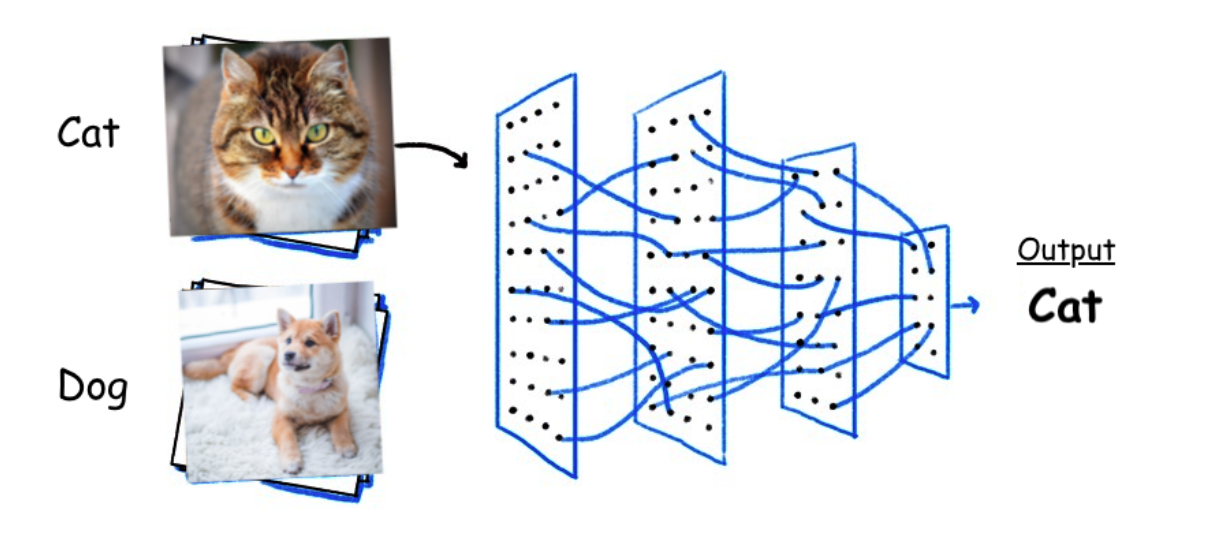
\includegraphics[scale=0.50]{classification_problem}
            \caption{Esempio classificazione binaria}
            \label{fig:figureClassification}
        \end{figure}
        Nel caso di un problema multiclasse, il numero di oggetti da identificare è maggiore di due, di conseguenza la rete sarà in grado di
        classificare $k>2$ classi.
    \section{MLP}\label{sec:mlp}
        Il Multilayer Perceptron è una struttura di rete basata sul perceptron, ma utilizzando più livelli.\\
        Ogni livello è costituito da dei "neuroni" che hanno la funzione di Perceptron, cioè quello di fornire un valore in uscita dati dei valori di ingresso, il quale servirà per i successivi layer. \\
        I layer possono essere distinti principalmente in tre categorie:
        \begin{itemize}
            \item Input Layer: composta dai nostri dati in ingresso.
            Il numero dei "neuroni" iniziali è dettato dal numero di features di cui abbiamo a disposizione.
            \item Hidden Layers: i layers "nascosti", dove effettivamente vengono processati i dati dai vari neuroni.
            Possono essere esserci più hidden layer in base al tipo di problema, e questi possono variare anche nel numero di neuroni.
            \item Output Layer: una volta che i dati vengono elaborati, la rete fornisce in uscita un predizione della categorizzazione.
        \end{itemize}
        Per i nostri esempi è sufficiente avere un unico hidden layer.
        \begin{figure}[H]
            \centering
            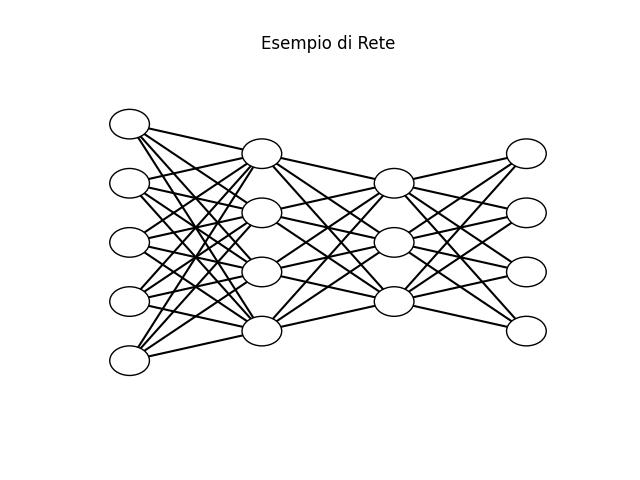
\includegraphics[scale=0.50]{neural_network}
            \caption{Esempio di Rete MLP Multiclasse}
            \label{fig:figure1}
        \end{figure}
        \subsection{BackPropagation}\label{subsec:backpropagation}
            Per l'apprendimento della rete utilizziamo l'algoritmo di backpropagation composto da due parti: una forward dove viene presentato un osservazione alla rete e successivamente calcolato il valore di uscita con determinazione dell'errore,
            e una backward dove l'errore calcolato dalla forward viene propagata all'indietro verso tutti i layers.
            In quest'ultima fase i pesi di tutti i layer vengono aggiustati per ottimizzare la classificazione per le successive osservazioni.\\
            Per l'ottimizzazione dei pesi: \begin{math} w_{t+1} = w_t - \gamma * \nabla_w L^{(i)}\end{math} \\
            Il parametro $\gamma$ rappresenta il grado di apprendimento della rete (learning rate).
        \subsection{Inizializzazione dei Parametri}\label{subsec:inizializzazione-dei-parametri}
            Nella fase d'inizializzazione di una rete è necessario inizializzare correttamente i parametri.\\
            Non è possibile inizializzare i pesi della rete a zero, dato che in questo caso la rete si fermerebbe al primo calcolo del gradiente.\\
            Esistono varie inizializzazioni, in questo elaborato ne vedremo in particolare due:
            \begin{itemize}
                \item Casuale: vengono randomizzati i valori iniziali
                \item Glorot: i valori saranno presi da distribuzione uniforme $U(-d, d)$ con $d=\sqrt{\frac{6}{padri_j + figli_j}}$
            \end{itemize}
        \subsection{Funzioni di attivazione}\label{subsec:funzioni-di-attivazione}
            \begin{itemize}
                \item Sigmoid: $\sigma(x) = \frac{1} {1 + e^{-x}}$
                \item Tanh: $tanh(x) = \frac{1 - e^{-2x}}{1 + e^{-2x}}$
                \item Relu: $Relu(x) = max(0, x)$
            \end{itemize}
        \subsubsection{Softmax}
            Utilizziamo anche la funzione di attivazione Softmax che sarà necessaria per mappare il vettore delle varie predizioni
            in un vettore $\theta$ tale che:
            $\sum\limits_j\theta_j = 1$\\
            Softmax: $\theta_{j} = \left\frac{e^{v_{j}}}{ \sum\limits_{r} e^{v_{j}}} \right r = 1,\dots,k$ con k = numero di classi
        \subsection{Multiclass Cross Entropy}\label{subsec:multiclass-cross-entropy}
            Per il caso multiclasse utilizziamo la funzione di loss: $l(\theta, y)=-\frac{1}{n}\sum_{j=1}^k{y_j}\log\theta{}_j$ con n = osservazioni.
        \subsection{Metodo del gradiente stocastico}\label{subsec:metodo-del-gradiente-stocastico}
            La parte critica dell'algoritmo backpropagation è il calcolo del gradiente, sopratutto quando il dataset è relativamente grande.\\
            Per risolvere questo problema possiamo adottare diverse strategie: una di queste è l'SGD (Stochastic Gradient Descent) che è il metodo utilizzato all'interno dell'elaborato per il passaggio dei dati del dataset.\\
            Preso un dataset, randomizziamo le varie osservazioni e da questo preleviamo un singolo indice i dal quale poi verrà calcolato la predizione e il suo relativo errore. \\
            Successivamente, preleveremo un altro indice per rieseguire il calcolo, fino a che non completeremo il dataset.\\
            L'iterazione di tutto il dataset si chiama epoca. \\
            Questo metodo permette di aumentare la velocità del calcolo del gradiente rispetto al Gradient Descent, cioè il passaggio dell'intero dataset. \\
            Un ultimo metodo che è possibile utilizzare è il Minibatch che consiste nell'iterazione di un range di indici (range = batch-size) alla volta fino al completamento del dataset. \\
            Se il range che utilizziamo per il minibatch è uguale al numero di tutto il dataset, otteniamo il Gradient Descent, se invece è uguale a uno riotteniamo il metodo del gradiente stocastico.\\
            L' SDG è più efficiente del gradient descent perché ottimizza i tempi dovuti al calcolo del gradiente, ma con lo svantaggio di essere meno preciso nella valutazione dell'errore.
            Il minibatch è il metodo che riesce a coniugare una migliore precisione con una maggiore velocità (a discapito di una maggiore implementazione).
    \section{Dataset}\label{sec:dataset}
        I dataset utilizzati sono stati presi dal sito: \href{https://archive-beta.ics.uci.edu/}{https://archive-beta.ics.uci.edu/} \\
        Entrambi i dataset hanno un numero di classi maggiori di 3, e numero di osservazioni maggiori di 5000. \\
        Il primo dataset utilizzato consiste nell'individuare, dati i features, se una macchina è soggetta a qualche tipo di malfunzionamento:
        \begin{itemize}
            \item numero di features = 5
            \item numero di classi = 4
            \item numero di osservazioni = 10000
        \end{itemize}
        Il secondo dataset è una classificazione di rane in base alle caratteristiche fornite in input:
        \begin{itemize}
            \item numero di features = 21
            \item numero di classi = 10
            \item numero di osservazioni = 7195
        \end{itemize}
        Di queste osservazioni ne vengano estrapolate circa milla per il validation set.
    \section{Valori Attesi}\label{sec:valori-attesi}
        Per come è stata progettata la nostra architettura, ci aspetteremo che la rete abbia una accuratezza peggiore nelle prime iterazioni dato che necessita di informazioni per l'apprendimento.
        Nelle successive iterazioni, la rete sarà in grado di apprendere molto di più migliorando quindi la precisione nella classificazione.
        Più sono i dati e il numero di epoche, più la rete sarà accurata nella classificazione.
    \section{Risultati}\label{sec:risultati}
        \subsection{Dataset 1 - Fallimento delle macchine.}\label{subsec:dataset-1}
            Sono stati presi 9000 osservazioni per 50 epoche per l'apprendimento della rete, con un learning rate pari a 0.0001.
            Validation set: Le restanti osservazioni, circa 1000, sono state utilizzate per il validation set:
            \begin{figure}[H]
                \centering
                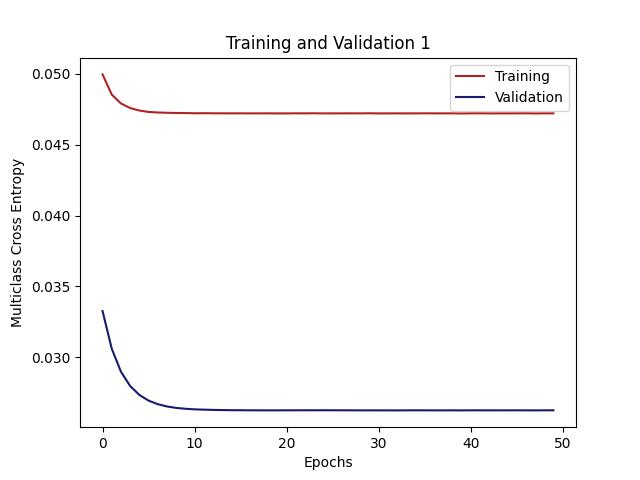
\includegraphics[scale=0.50]{lossval1}
                \caption{Cross Entropy sul training set e validation set}
                \label{fig:figure3}
            \end{figure}
            Il valore di predizione inizialmente si rivela già notevolmente basso già dalle prime iterazioni per poi arrivare alla conversione.
            Sia che per il training set che per il validation set possiamo che notare che entrambi i grafici tendono a diminuire.
            Questo ci mostra che la rete apprende bene e non va in over-fitting.
        \subsection{Dataset 2 - Classificazione delle rane}\label{subsec:dataset-2---classificazione-delle-rane}
            Sono stati presi 6000 osservazioni per 50 epoche per l'apprendimento della rete, con learning rate pari a 0.0001.
            Validation: Le restanti osservazioni, circa 1000, sono state utilizzate per il validation set:
            \begin{figure}[H]
                \centering
                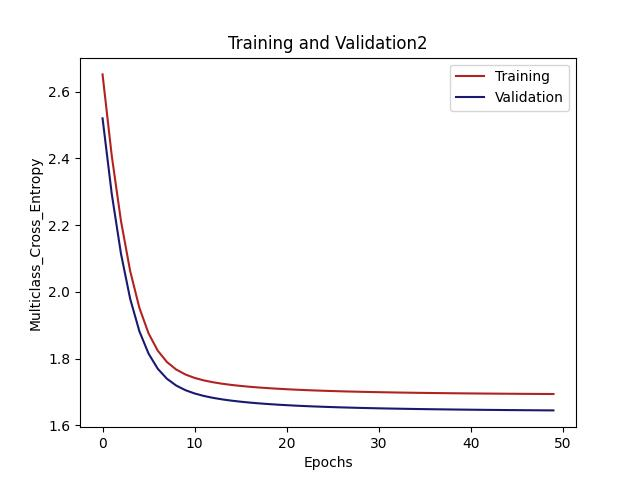
\includegraphics[scale=0.50]{lossval2}
                \caption{Cross Entropy sul training set e validation set}
                \label{fig:figure4}
            \end{figure}
            \newpage
            Come è possibile vedere, in questo caso, il valore iniziale di loss è più alto rispetto al primo dateset dato che il numero di classi è più alto e il numero di osservazione è minore.
            Nonostante tutto, la rete converge fino al valore più basso.
            Anche in questo caso, il training set e il validation set tendono a diminuire, non andando in over-fitting.
    \section{Conclusioni}\label{sec:conclusioni}
        Come abbiamo potuto osservare dai grafici, la rete una volta che apprende dai dati riesce ad apprendere sempre di più fino ad arrivare alla convergenza.
        Per entrambi i dataset sia il training set e il validation set diminuiscono, non andando in over-fitting, mostrandoci che il modello architetturale descritto è un buon modello.
        Per diminuire l'errore nel dataset 2 sarà necessario fornire un maggior numero di osservazioni per far apprendere meglio la rete data il grande numero di classi da identificare.
    \section{Caratteristiche Terminale}\label{sec:caratteristiche-terminale}
        Il terminale su cui sono state svolte le prove:
        \begin{itemize}
            \item Sistema Operativo: Windows 11 PRO
            \item Processore: Intel I5-8600K
            \item Scheda Video: Nvdia GEFORCE 1050-Ti
            \item Ram: 16GB DDR4 3600MHz
        \end{itemize}
    \section{Riferimenti e Letture}\label{sec:riferimenti-e-letture}
        \begin{itemize}
            \item \href{https://rstudio-pubs-static.s3.amazonaws.com/337306_79a7966fad184532ab3ad66b322fe96e.html#backpropagation}{backpropagation}
            \item \href{https://archive-beta.ics.uci.edu/} {archivio datasets}
            \item \href{https://gist.github.com/craffel/2d727968c3aaebd10359} {metodo per il plot della rete}
        \end{itemize}
\end{document}